\chapter{Evaluation}\label{cha:evaluation}

Envoy is designed based on assumptions about a platform that does not yet exist. This limits how the system can be evaluated in two ways. The first is scalability. While common bottlenecks can be avoided and the architecture examined for potential scalability limitations, a system without a large-scale implementation can never be fully tested for issues that only appear at large scales. The best that can be achieved is to identify the most likely sources of problems and extrapolate the results of testing on a smaller scale. The architecture can also be evaluated against assumptions about the workloads it is intended to support, which leads to the second limitation: workloads cannot be accurately forecast. Predicting and simulating client access patterns is a difficult problem even for existing environments \cite{ganger95}, and the problem is amplified for service clusters. As a general purpose platform, service clusters are intended to support a wide range of existing workloads and to enable a flourishing ecosystem of computation services that create entirely new workloads. The design and the evaluation must necessarily rely on assumptions about how the system will be used, and those assumptions limit the applicability of the results.

In this chapter I evaluate the Envoy prototype with three principal goals: to measure the impact of specific design choices, including the basic distributed organisation and cache layout, to assess the scalability of the system, and to evaluate Envoy's ability to support the types of workloads expected in service clusters.

\section{Methodology}

The absence of a realistically sized service cluster limits the scope of system-level testing and the usefulness of many application-level results. The performance side-effects of interacting components and the access patterns of different clients are particularly difficult to predict. The performance characteristics of the storage layer depend on design elements and implementation choices beyond the scope of this dissertation. These factors combined with the poor public availability of many comparable systems limit direct comparisons to previous work.

Building and evaluating a prototype of the Envoy file system is not a futile exercise, however. The artefact may reveal little about real-world usage and behaviour, but measuring it can still do much to justify or condemn the design. The remainder of this section outlines assumptions about service clusters that influence the design, how the design reflects them, and how measuring the prototype helps to evaluate the decisions made.

\subsection{Evaluation goals}

\subsubsection{Independent clients}

* independent boot images, and dynamic transfers to keep them independent as much as possible
* scalability

\subsubsection{Shared images}

* dynamic transfers--sharing should only happen when there is actual sharing
* keep access to a single cache even when sharing--compare dist lock (flushing to storage layer when token is transferred) to the extra network hop using a single cache

\subsubsection{Scalability}

* assumption is that it is scalable?  more of an argument than an evaluation: envoys don't interact unless they are sharing something (including a border), storage layer mostly consulted for writes(?), but number of spindles grows with the size of the cluster anyway
* what is actually tested here to prove this?

\subsubsection{Expected workloads}

* does the dynamic algorithm work?
* does it serve isolation clients
* does it serve shared clients
* what are the weaknesses


Envoy assumes that skewed file access distributions will continue to be a feature of future workloads just as it is of current workloads. Furthermore, it uses template images to encourage implicit sharing between clients. Both factors call for caching, but the latter in particular makes caching at the machine level beneficial, since all clients hosted on a machine can inherit data from common image templates and profitably share a cache, even in the absense of any explicit relationship between the clients.

Caching is managed at the machine level, with a single in-memory and on-disk pool for all of the clients hosted on that node. Client behaviour cannot always be predicted, but the tradeoffs of this cache model can be evaluated. \secref{sec:architectural-costs} compares the performance of the in-memory and on-disk caches with access to the uncached storage layer, and also discusses the cost of a single machine-level cache over per-client caching. These measurements compare the performance gains and losses that can be directly attributed to the cache model, and \secref{sec:quantifying-sharing} applies the results to the assumed model of implicit sharing between clients using the same template image.

* validate the basic goals envoy tries to achieve
* overheads of data paths, justify cache design and territory system
* aggregate caching benefits and costs


\subsection{Test environment}

\subsubsection{Hardware}

\subsubsection{Benchmarks}

Linux source tree: stats about it

untar -- write test

tar > /dev/null -- read test

rsync -- 2nd read test

Bonnie: info about it

\section{Independent clients}

Much of the complexity in distributed file system design is related to data sharing, but sharing is less common than individual clients accessing private data. A service derived from a standalone machine typically requires a private boot image, and lightweight fork operations in Envoy encourage the cloning of entire images for private use by related and unrelated service instances.

To succeed as a distributed file system on a large scale, Envoy must provide a useful service to isolated clients that obviates the need for additional storage services for most clients. While there is no technical or administrative distinction between private and shared images, Envoy's design and runtime behaviour under these two conditions can be evaluated seperately. This section focuses on Envoy's performance and behaviour in the absense of sharing.

\subsection{Performance}

The prototype is not optimized, and absolute performance is not the focus of this evaluation. Nevertheless, it is helpful to establish baseline performance numbers to show that Envoy is viable as a file system. For context, the results are compared to \texttt{npfs}, a multi-threaded userspace 9p server, and \texttt{unfsd}, a single-threaded userspace NFS server. Userspace servers have additional overhead when compared to kernel implementations, but the penalty is assumed to be similar for all of the implementations tested. Standard benchmarks do a poor job of isolating the costs involved in Envoy's data paths, and most of the evaluation in this chapter eschews them in favor of more controlled tests, but this section starts with the Bonnie benchmark to provide some raw performance figures comparable to those from other systems.

\begin{figure}[t]
\centering
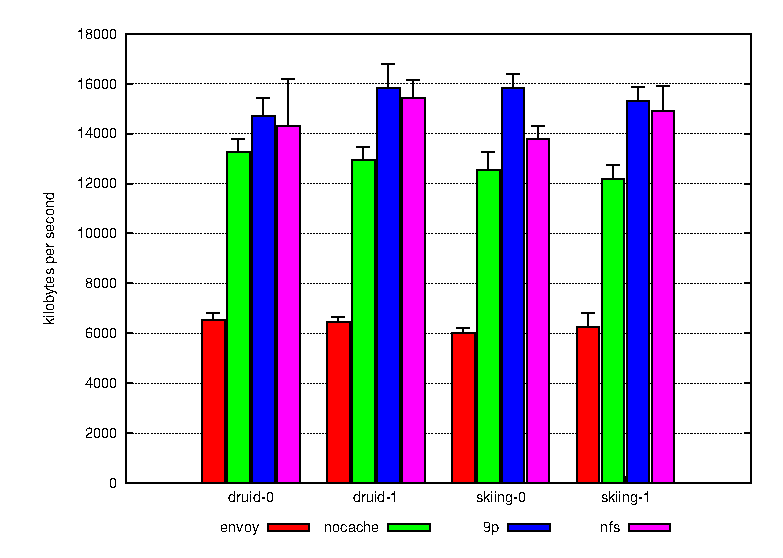
\includegraphics[width=\figwidth]{figures/bonnie-write}
\caption[Bonnie benchmark results for block writes]{Bonnie benchmark results for block writes on a 2GB dataset. Results for Envoy, Envoy with no persistent cache, a userspace 9p server, and a userspace nfs server are compared. Error bars show the standard deviation over ten runs.}
\label{fig:bonnie-write}
\end{figure}

\figref{fig:bonnie-write} shows the block write results of the Bonnie benchmark on a 2GB dataset. The four clusters show different client locations. druid-0 hosts the envoy that owns the territory for the Envoy results (displayed with and without the persistent cache enabled), and runs the server for the 9p and nfs results. druid-1 is a client VM on the same machine, skiing-0 the administrative VM on a remote machine (which also hosts an envoy instance), and skiing-1 is a client domain on the remote machine. Both druid-0 and skiing-0 host storage server instances with complete replicas of all storage objects.

Envoy's persistent cache creates a large penalty for writes, but this is a worst-case result. Data must be written twice since a storage instance is located on the same machine using the same hard drive, in addition to the storage replica on the skiing-0. Disabling the persistent cache boosts write performance considerably, putting it on par with the other servers. Writing it twice on two machines incurs some overhead, but it is acceptable for the simplistic storage server used in the prototype. 9p is generally a bit faster than NFS because of its simpler protocol and larger message size, but in this simple test waiting for the disk dominates all of the servers.

\begin{figure}[t]
\centering
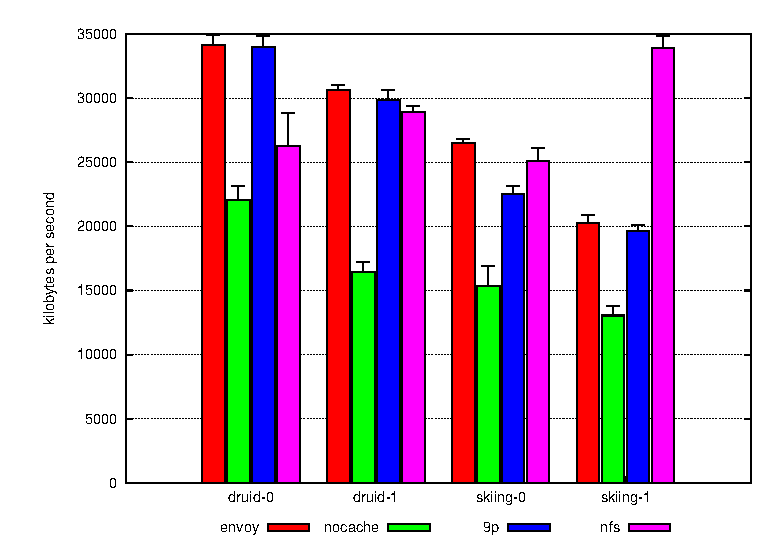
\includegraphics[width=\figwidth]{figures/bonnie-read}
\caption[Bonnie benchmark results for block reads]{Bonnie benchmark results for block reads on a 2GB dataset. Results for Envoy, Envoy with no persistent cache, a userspace 9p server, and a userspace nfs server are compared. Error bars show the standard deviation over ten runs.}
\label{fig:bonnie-read}
\end{figure}

\figref{fig:bonnie-read} shows the block read results from the same benchmark. The persistent cache does not incur a double-access penalty as in the write case, so it improves the results. All data is present in the persistent cache (though the dataset is too large for the in-memory cache), so the Envoy results are similar to the 9p results in this test. Disabling the persistent cache forces retrieval from the storage servers, and each request is randomly directed to one of the two replicas.

The NFS numbers are more confusing. This is probably due to the interactions between the client-side cache and the server cache. The cache was flushed before each run by deleting all files and remounting the partition, the server processes were restarted, and clients were remounted, but each run of the benchmark executes a series of tests in succession without any explicit \texttt{sync} calls. The interaction of two levels of delayed write-back caching, particularly when both are part of the same buffer cache on druid-0, could explain the curious results. The behaviour of NFS is not the focus of this evaluation, however.

\begin{figure}[t]
\centering
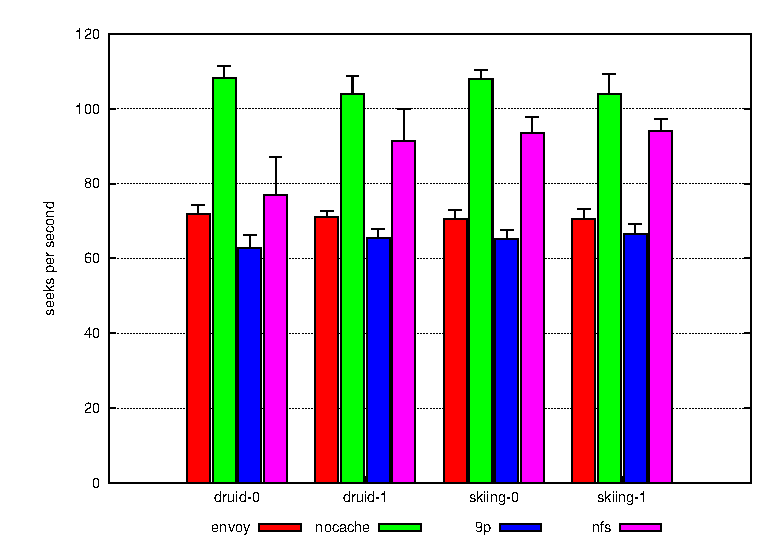
\includegraphics[width=\figwidth]{figures/bonnie-seek}
\caption[Bonnie benchmark results for random seeks]{Bonnie benchmark results for random seeks on a 2GB dataset. Results for Envoy, Envoy with no persistent cache, a userspace 9p server, and a userspace nfs server are compared. Error bars show the standard deviation over ten runs.}
\label{fig:bonnie-seek}
\end{figure}

\figref{fig:bonnie-seek} shows the results of the concurrent random seek test in Bonnie. Disabling the persistent cache helps Envoy because concurrent requests are randomly directed to two different disks, and the effective cache size is much larger. With no persistent cache, the memory on druid-0 and skiing-0 is used mostly by the storage server cache, but when the persistent cache is enabled, only druid-0 contributes memory and it is split between its storage instance and the persistent cache. The prototype only allows one outstanding request per storage object, so seek penalties are not significantly reduced by using two disks. NFS probably also benefits from combining the client-side cache with the server cache. In Envoy's intended environment, client cache sizes would be smaller and server caches larger to encourage sharing, but this benchmark only acts from a single client.

\subsection{Architecture}\label{sec:architectural-costs}

An important goal of the Envoy design is to localize data and metadata control when possible, and minimize the involvement of disinterested nodes when not possible. Private images are always controlled by the envoy instance on the same machine as the client using it, and territories in shared images are managed by the most active participant. Besides reducing collateral impact in a bid to improve scalability, localizing control and caching has direct performance benefits for clients.

As described in \secref{sec:data-paths}, requests follow one of several paths to completion depending on whether or not the required data is cached and whether ownership is local or remote. The worst case for local or remote ownership is when the data must be retrieved from the storage layer. \figref{fig:envoy-cold} shows the results 

\figref{fig:envoy-tar} uses the \texttt{tar} test to compare these different paths. \texttt{druid-0} hosts the envoy service that owns the data being read, and \texttt{druid-1} is a client on the same machine. Similarly, \texttt{skiing-0} hosts a remote envoy instance, and \texttt{skiing-1} is a client on the same machine. The first bar, labeled ``hot'', shows the time required to read a Linux source tree that is in the server's in-memory cache. The ``warm'' results read the data from the persistent cache, requiring validation with the storage layer but no data transfer, while ``cold'' results require transferring everything from the storage layer.

userspace NFS

userspace 9p

envoy local dom0

envoy local domU

envoy remote dom0

envoy remote domU

cache: cold vs warm vs hot

If the goal is to get stuff as local as possible, quantify the benefits of achieving that. Measure the overheads of data paths and cache decisions.

\subsubsection{Local impact}

Independence of private images

\subsection{Cache}

\subsubsection{Quantifying sharing}\label{sec:quantifying-sharing}

SUSE10 upgrade, install services

compare image overlap

boot two related images (one cold and other warm) and compare with the same test for identical images

show sharing: boot one VM from cold cache, boot another based on same template

\section{Shared images}

\subsection{Territory migration}

cost of transferring state

two machines with kernel in hot cache, do read test while transferring ownership back and forth between them

\subsection{Dynamic behaviour}

Test dynamic territory management, less about performance than behaviour

probabilistic traffic driven to overlapping areas

shared image with (independent) home directories

2 log files in one directory

producer-consumer

\subsubsection{Sharing application}
something that shares in a complex but predictable fashion

\section{Image operations}

\subsubsection{Forks}

cheap and fast---these always happen from a read-only snapshot

\subsubsection{Snapshots}

single territory

untar the kernel while a bunch of snapshots happen and measure the impact

snapshots with many territories

\section{Summary}
